
\chapter {Achievement}
\renewcommand{\chaptername}{Chapter}

~~~~~This chapter discusses the implementation of the toolkit’s components.

We begin by presenting the development tools supporting the choices made then proceed to the software environment and end the chapter by displaying some interfaces of the achieved work.
\section{Developing Environment}


\subsection {Hardware Environment}
All along this project, with a reliable Internet connection, we used a computer with characteristics provided in Table \ref{computers}


\begin{table}[!htbp]

\begin{center}
\begin{tabular}{| m{5em} | m{6cm} | }
\hline
Processor & i7 2.7 GHz \\ 
\hline
Ram & 8 GB\\ 
\hline
Hard Drive & 1 TB  \\ 
\hline
Operating system & SecurityOnion 14.04 64Bits
\hline
\end{tabular}
\label{computers}
\end{center}
\caption{Characteristic of the used computer}
\end{table}


\subsection {Software Environment}
In this part, we list the different software products we used throughout the development of our application : 


%-----------------------------------------------


  
\begin{itemize}[label=\ding{112}]
  
\item\textit{Ruby Mine}

A smart editor that enables the user to produce high-quality code more efficiently, thanks to first-class support for Ruby and Rails, JavaScript and CoffeeScript, ERB and HAML, CSS and more.

Moreover, the programmer might take advantage of language specific-aware syntax \& error highlighting, code formatting, code completion, and quick documentation.
It only takes one click to switch to the declaration, super method, test, usages, implementation...
Automated yet safe refactorings are provided. They help clean the code and keep it more maintainable. Rails-aware refactorings help  performing project-wide changes: for example renaming a controller will also rename helper, views and tests. \cite{ruby}

Figure \ref{rubymine} shows an overview of RubyMine, which was the main editor we used throughout the programming phase. This software simplified the manipulation of the project's documents, syntax errors detection and server administration.
Furthermore, a few of its pre-configured features such as VCS management and included terminal were extremely proficient.

\begin{figure}[!htpb] 
\begin{center}
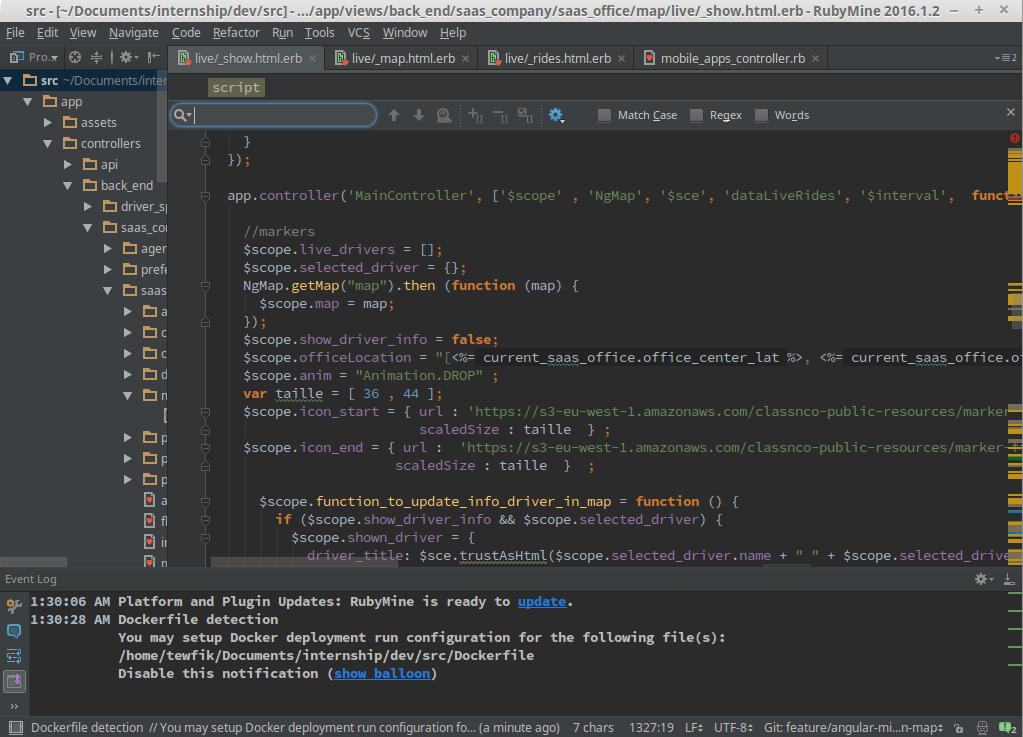
\includegraphics[width=6 in, height = 2 in]{images/rubymine.png}
\caption{RubyMine}
\label{rubymine}
\end{center}
\end{figure}



\item\textit{pgAdmin III}

pgAdmin is the most popular and feature rich Open Source administration and development platform for PostgreSQL, the most advanced Open Source database in the world. The application may be used on Linux, FreeBSD, Solaris, macOS and Windows platforms to manage PostgreSQL 9.2 and above running on any platform, as well as commercial and derived versions of PostgreSQL such as EDB Postgres Advanced Server.

pgAdmin is designed to answer the needs of all users, from writing simple SQL queries to developing complex databases. The graphical interface may be run on the desktop or on a web server and supports all common PostgreSQL features. The application includes a syntax highlighting SQL editor.

pgAdmin is developed by a community of PostgreSQL experts around the world. It is Free Software released under the PostgreSQL License. Figure \ref{pgAdmin} \cite{pgAdmin} unveils the welcome page of this software.

\begin{figure}[!htpb] 
\begin{center}
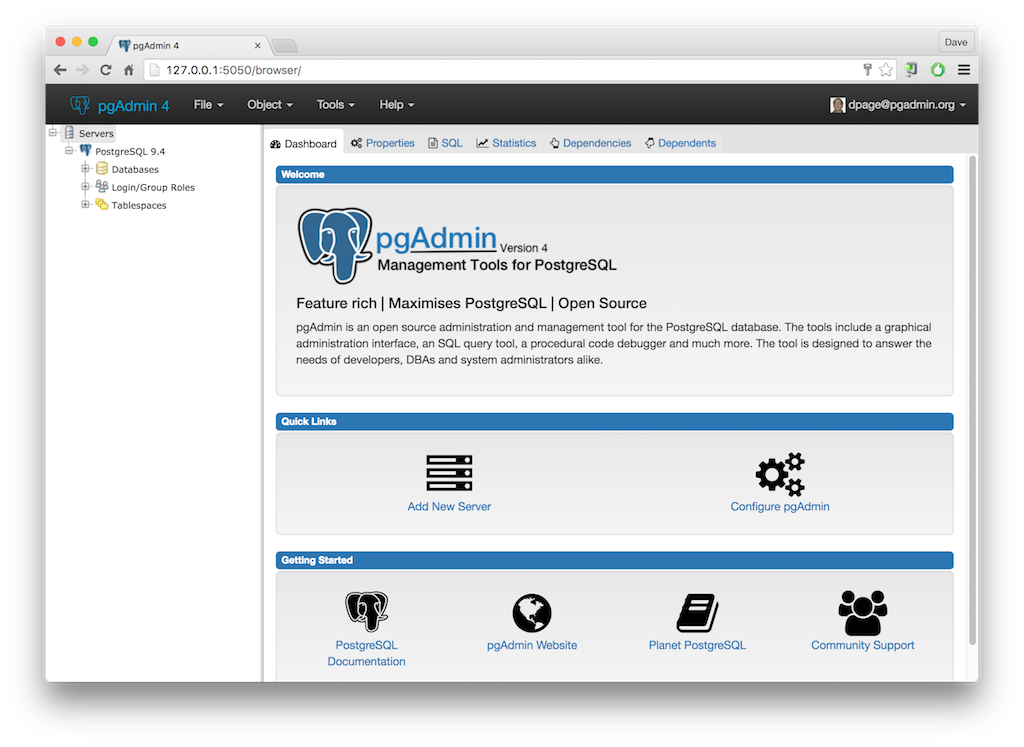
\includegraphics[width=6 in, height = 2 in]{images/pgAdmin.png}
\caption{ pgAdmin - Management Tools for PostgreSQL }
\label{pgAdmin}
\end{center}
\end{figure}

\item\textit{Draw.io}

draw.io is a free to use online diagramming application. Diagrams are then stored locally in order to edit them. We used this tool in order to draw various existing diagrams in the report. 

\item\textit{Chromium developer’s tools}

The Developer Tools, bundled and available in Chrome, grant web developers and programmers deep access into the internals of the browser and their web application.

The Developer Tools are heavily based on the WebKit Web Inspector, a part of the open source WebKit project.



Figure \ref{chrome_dev} shows an overview of the Developer Tools, points out its most popular and useful features. This tool helped us manipulating scripts, debugging as well as identifying any errors that might have occurred during the development process.

\begin{figure}[!htpb] 
\begin{center}
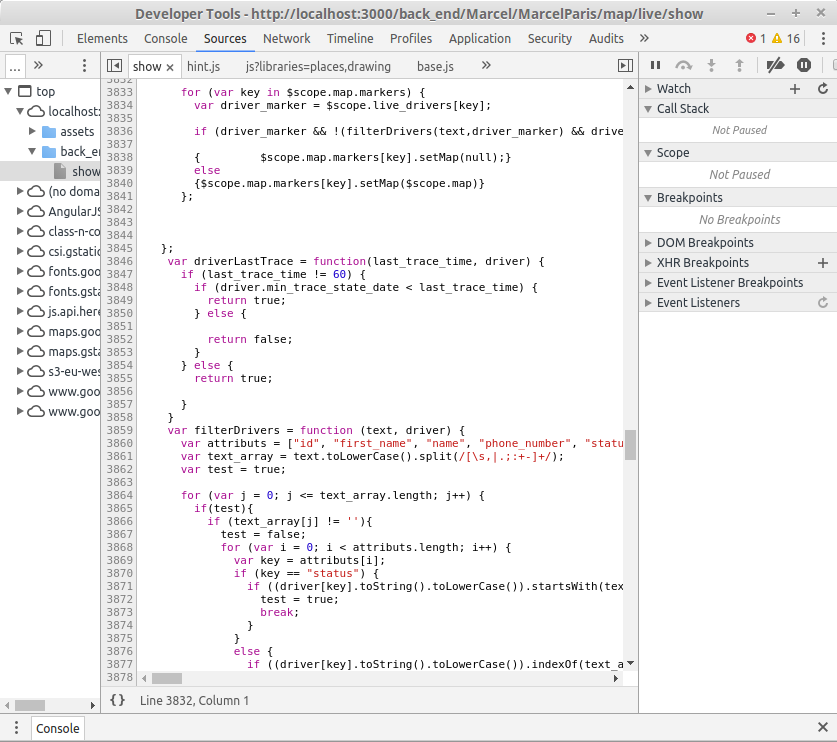
\includegraphics[width=6 in, height = 2 in]{images/chrome.png}
\caption{Chromium developer’s tools}
\label{chrome_dev}
\end{center}
\end{figure}~




%-------------------------------------
\end{itemize}



\section {Technical Choices}
In this section, we discuss the technical choices we made to achieve our application. We start
by presenting the languages used in the development of the project. Afterwards, we defend
our choice for the frameworks we used.
\subsection{Development Language}

The languages we used throughout the development phase are :
 \textbf{Shell} 

 \textbf{JavaScript } 
 
A scripting language object oriented mainly used in web browsers to add interactivity to HTML pages. In contrast to server-side languages (running on the site), JavaScript code is usually embedded directly into these pages since JS is an interpreted language meaning that scripts are executed without preliminary compilation. The standardized version of JavaScript is ECMAScript \cite{js}.

In our case, we resorted to using this programming language considering that angularJS 1.4.3 is written solely in Javascript.

\textbf{PL/pgSQL  }

PL/pgSQL (Procedural Language/PostgreSQL) is a procedural programming language supported by the PostgreSQL ORDBMS. It closely resembles Oracle's PL/SQL language.

PostgreSQL is an object-relational database management system (ORDBMS) based on POSTGRES, Version 4.2, developed at the University of California in the computer science department of Berkeley. 
In addition, PostgreSQL can be extended in several ways by the user, providing more power and flexibility.  \cite{postgres}

PostgreSQL can be used, modified and distributed by anyone for free thanks to its free licence. Regardless of these advantages, we opted for this choice since it has already been in use at the company.

\subsection{Development Framework}

The frameworks we used throughout the implementation stage are :

\begin{itemize}
\item \textbf{AngularJS } 

AngularJS is a Javascript framework. It allows the user to extend HTML vocabulary for his application. The resulting environment is extraordinarily expressive, readable and quick to develop. The main purpose of using AngularJS is promptly building responsive SPA. As a matter of fact, treating interactivity as a native component of HTML is one of the most efficient aspect of this framework.

The essential goal is building CRUD style business applications. Increasing the use of two-ways data bindings and dependency injections empowers the exploitation of angular.
Below are a few of the used modules in addition to the created ones :

\begin{itemize}[label=\ding{50}]

\item\textit{ng-map }

A module created by allenhwkim using different approach than the official module for google Maps Javascript API, since it exposes all original Google Maps V3 api to the user. It provides a simple API for diving into common map processing tasks such as setting itineraries, drawing markers, changing the type of the map, showing roads and more.. ng-map is used in the client side to ensure a fast representation process for each received ride information. Furthermore, customized markers according to the driver's type are easily incorporated into the map.


\item\textit{ui-grid }

A module created as part of AngularUI suite, the companion suite to the angularJS framework. It provides basically a data grid along with numerous features related to customizing the grid. Performing well with very large data sets as well as offering various fancy options elect it as the most suitable choice in our case. Hence, displaying wide range of ride information is handled easily by this module. Different columns adjusting options are offered as well through a user friendly and intuitive interface, while hiding the complexity of the processes.  


\item\textit{angular-animate}

Provides animation hooks for common directives such as ngRepeat, ngSwitch, and ngView, as well as custom directives via the \$animate service. These animation hooks are set in place to trigger animations during the life cycle of various directives and when triggered, will attempt to perform a CSS Transition, CSS Keyframe Animation or a JavaScript callback Animation (depending on if an animation is placed on the given directive). Animations can be placed using vanilla CSS by following the naming conventions set in place by AngularJS or with JavaScript code when it's defined as a factory \cite{ngAnimate}.

We ought to utilise ng-animate in contemplation of satisfying non functional requirements concerning the ergonomy of the application. 
Therefore, the SaaS office would enjoy a pleasant experience and dynamic interactions while manoeuvring through the application. 

\end{itemize}

\item \textbf{Twitter Bootstrap } 

Sleek, intuitive, and powerful front-end framework for faster and easier web development.

\end{itemize}


%--------------------------interfaces 
\section{Achieved Work}

In order to be successful, an application should adopt fluent and easy to follow instructions.

Especially in our case, since it consists of a SaaS product, each client insists on following his own preferences. Nevertheless, our achieved work must provide generic features that are common to all the clients. In order to ensure their satisfaction, we present in this section the different aspects of our SPA that they can easily manipulate.

\subsection{Main Page }

For starters, the SaaS office must sign in to the BackEnd workspace after inserting his credentials. Once authenticated, the main page is loaded once for all as shown in Figure \ref{int0}. He may operate on this single page application and benefit from all of its features without reloading it.

Intuitive tabs are available to ensure the ease of the use. These tabs are customizable as the user can modify their dimension, place and color as he pleases. 
The main three tabs of our component reside in 'The Map', 'The ride table' and 'The Ride Information'.

Each tab possess its own independent particularities. Yet, they are thoroughly interconnected as a constant communication between them is established.



\begin{figure}[!htbp] 
\begin{center}
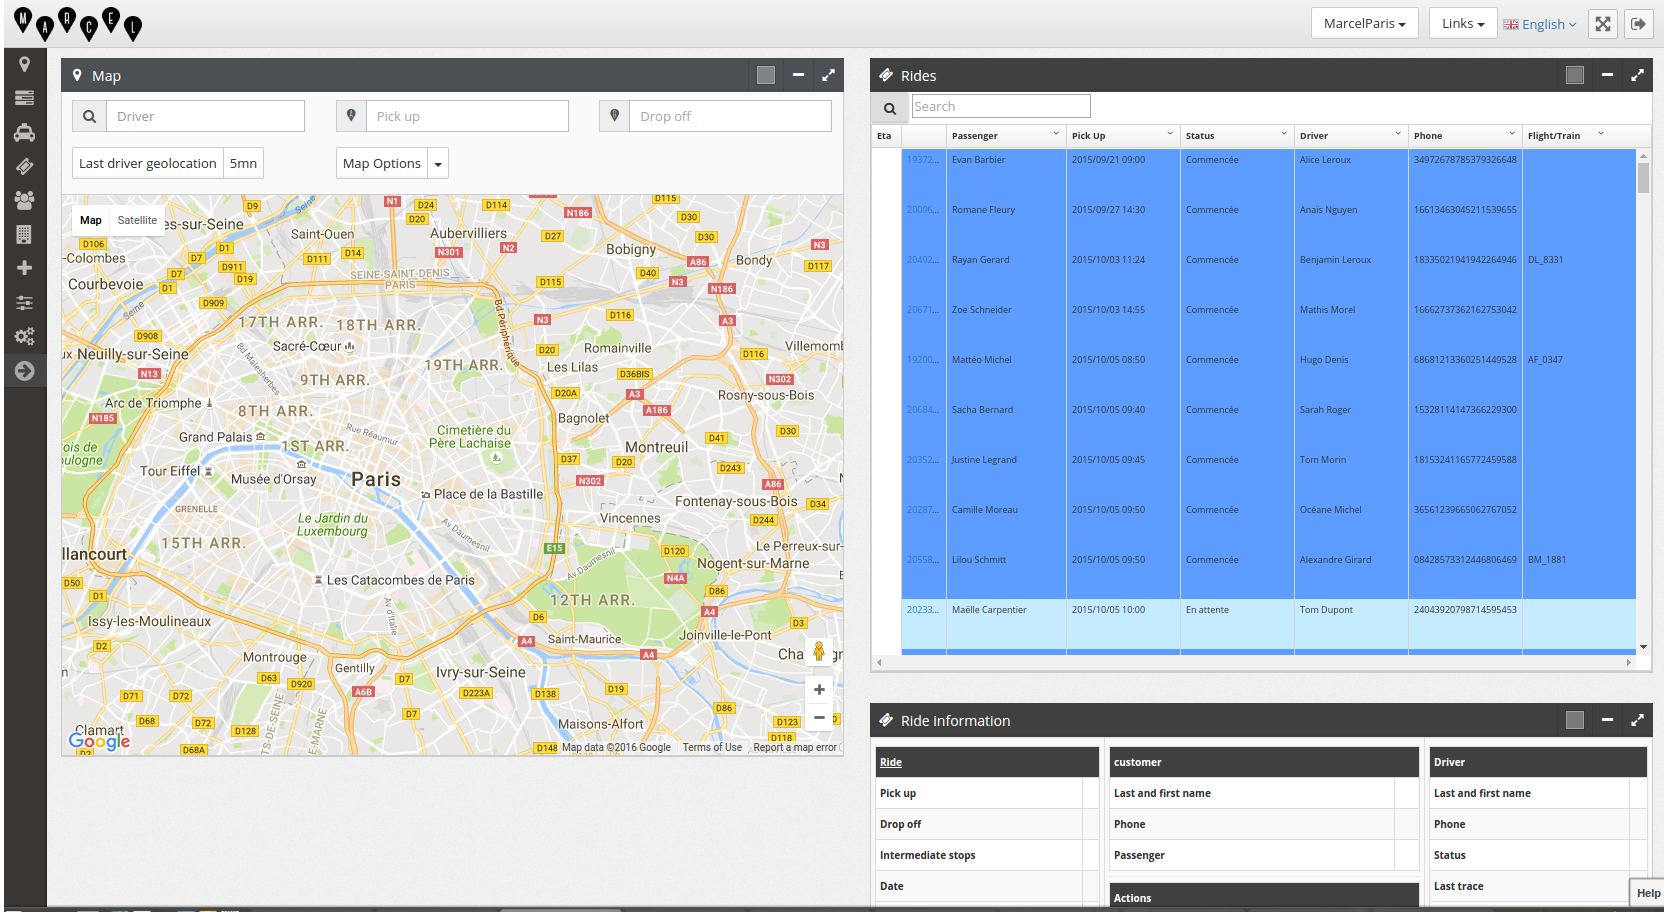
\includegraphics[width=6.6 in , height=4.5 in]{images/achievement/0.png}
\caption{Interface of the main page}
\label{int0}
\end{center}
\end{figure}~


\subsection{The Map }

The map generated by google proffers to the user all of the main aspects concerning the manipulation of the map. For instance, the user may zoom in and out and navigate through the map.
Furthermore, the user has the ability to customize the style of the map according to his preferences. The first step is to select the map styles menu that enlists the different customized styles as well as the main map modes. Figure  \ref{int2} demonstrates an example of the customized styles called 'nightvision'.

Moreover, the map's type chosen once by the user is registered in the browser session storage. So that after each reload, that saved value is assigned automatically to the map.


\begin{figure}[!htbp] 
\begin{center}
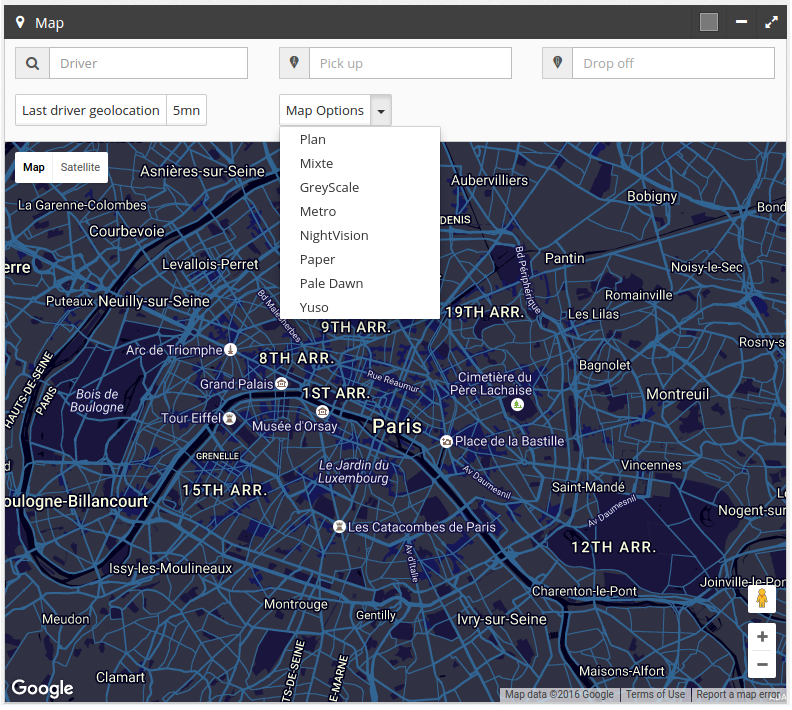
\includegraphics[width=6 in]{images/achievement/2.png}
\caption{Interface of the map tab}
\label{int2}
\end{center}
\end{figure}~

\subsection{Rides' Table }

Concerning the table of booked rides, it is filled instantly after the reload and the user may navigate through its rows.
Each row has a background color based on the status of the rides. The different colors are not specified since this was not a generic task. As a matter of fact, each client prefer different colors associated to the rides' status.

Figure \ref{int3} proves that only necessary data are displayed. These data concern the passenger's name, the pick-up time, the driver's name and phone number, the ride reference...

\begin{figure}[!htbp] 
\begin{center}
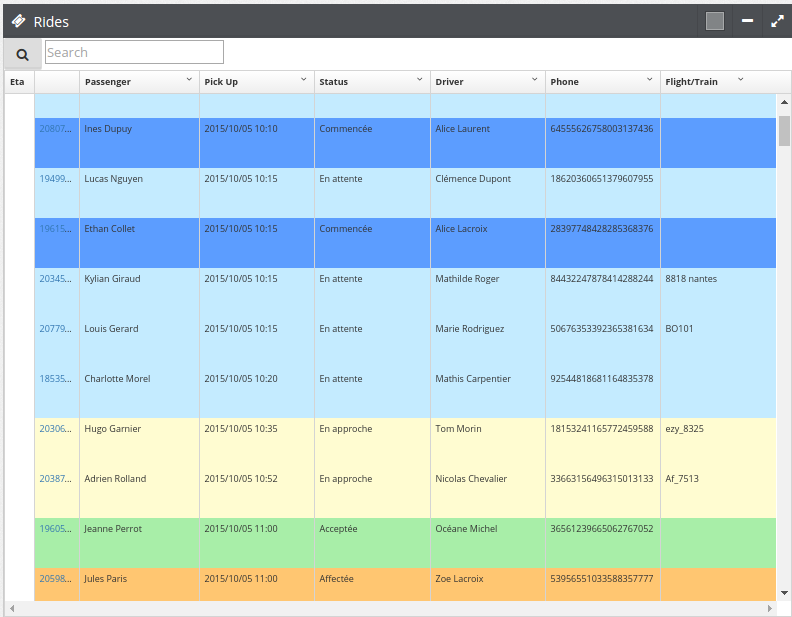
\includegraphics[width=6 in]{images/achievement/3.png}
\caption{Interface of the rides' table}
\label{int3}
\end{center}
\end{figure}~


After organizing the columns whether by descending or ascending order, the user is also able to search through the table.

Figure \ref{int4} shows that only two rows were left in the table according to the searched term. It is important to point out that the search process implies not only the passenger's name, but all of the columns. 
Hence, a view of only on-going rides is simply possible. Once the search term is to be inserted, the filter mechanism starts immediately.

\begin{figure}[!htbp] 
\begin{center}
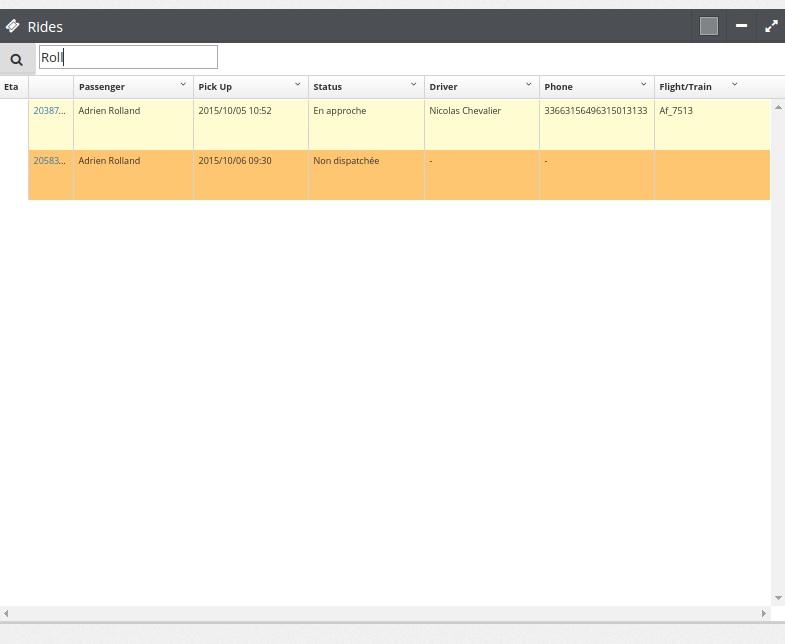
\includegraphics[width=4.5 in]{images/achievement/4.png}
\caption{Interface of the rides' table filtered }
\label{int4}
\end{center}
\end{figure}~



\subsection{Select a Ride  }

Taking a closer look at the rides' table, essential facts about the itinerary seem to be missing. Furthermore, more detailed information are being hidden in order to ensure the readability of the table.
Thus, the user is capable of reviewing the totality of information about a certain ride once he selects it. 
Simply put, the user ought to select a row in order for its background-color to change, but most importantly, further hidden data are to be shown instantly.

At this point, the user has the privilege to visualize a clear and obvious itinerary as shown in Figure \ref{int5}. In fact, the path is drawn immediately on the map with markers of the arrival and departure positions. The map is automatically zoomed into the ranged zone of the correspondent path.


\begin{figure}[!htbp] 
\begin{center}
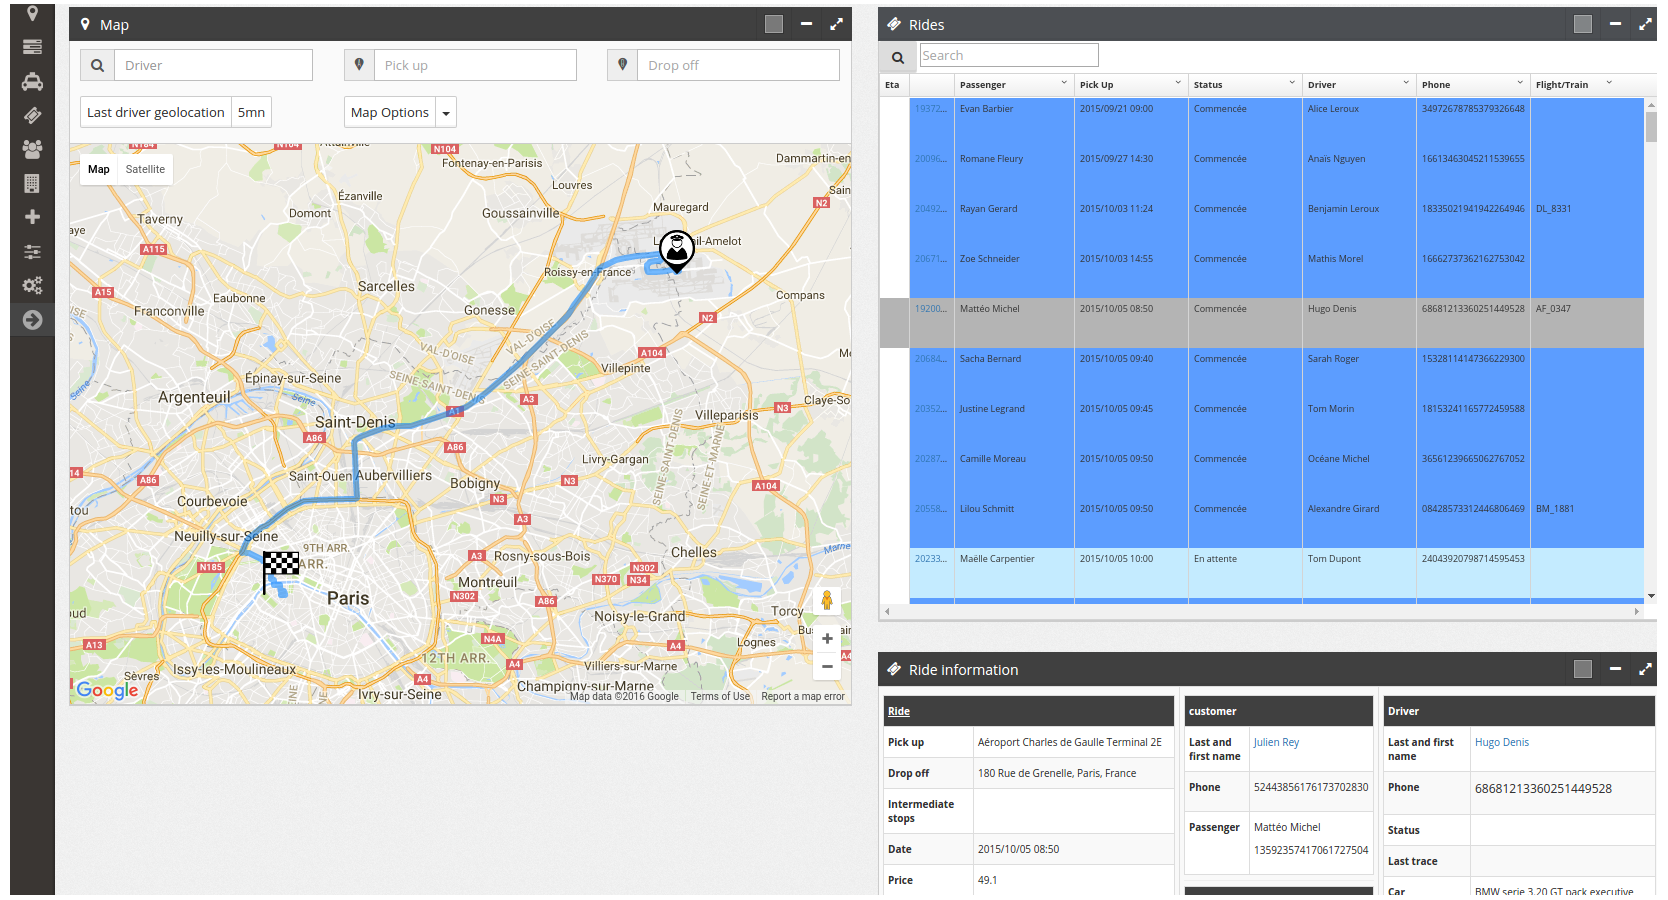
\includegraphics[width=6 in]{images/achievement/5.png}
\caption{Interface of the ride's itinerary }
\label{int5}
\end{center}
\end{figure}~


Simultaneously, the ride's information tab is instantly filled with information according the ride selected. Figure \ref{int6} shows a simple overview of the consequences of the user's click. Highlighted data such as the driver's  name and so are not just raw pieces of data. However, they constitute hyperlinks that enable the user to view their correspondent, full options, profiles. 

In addition to that, the user is only allowed to select one row at a time. Therefore, while selecting another ride, the same process is achieved again right away.



\begin{figure}[!htbp] 
\begin{center}
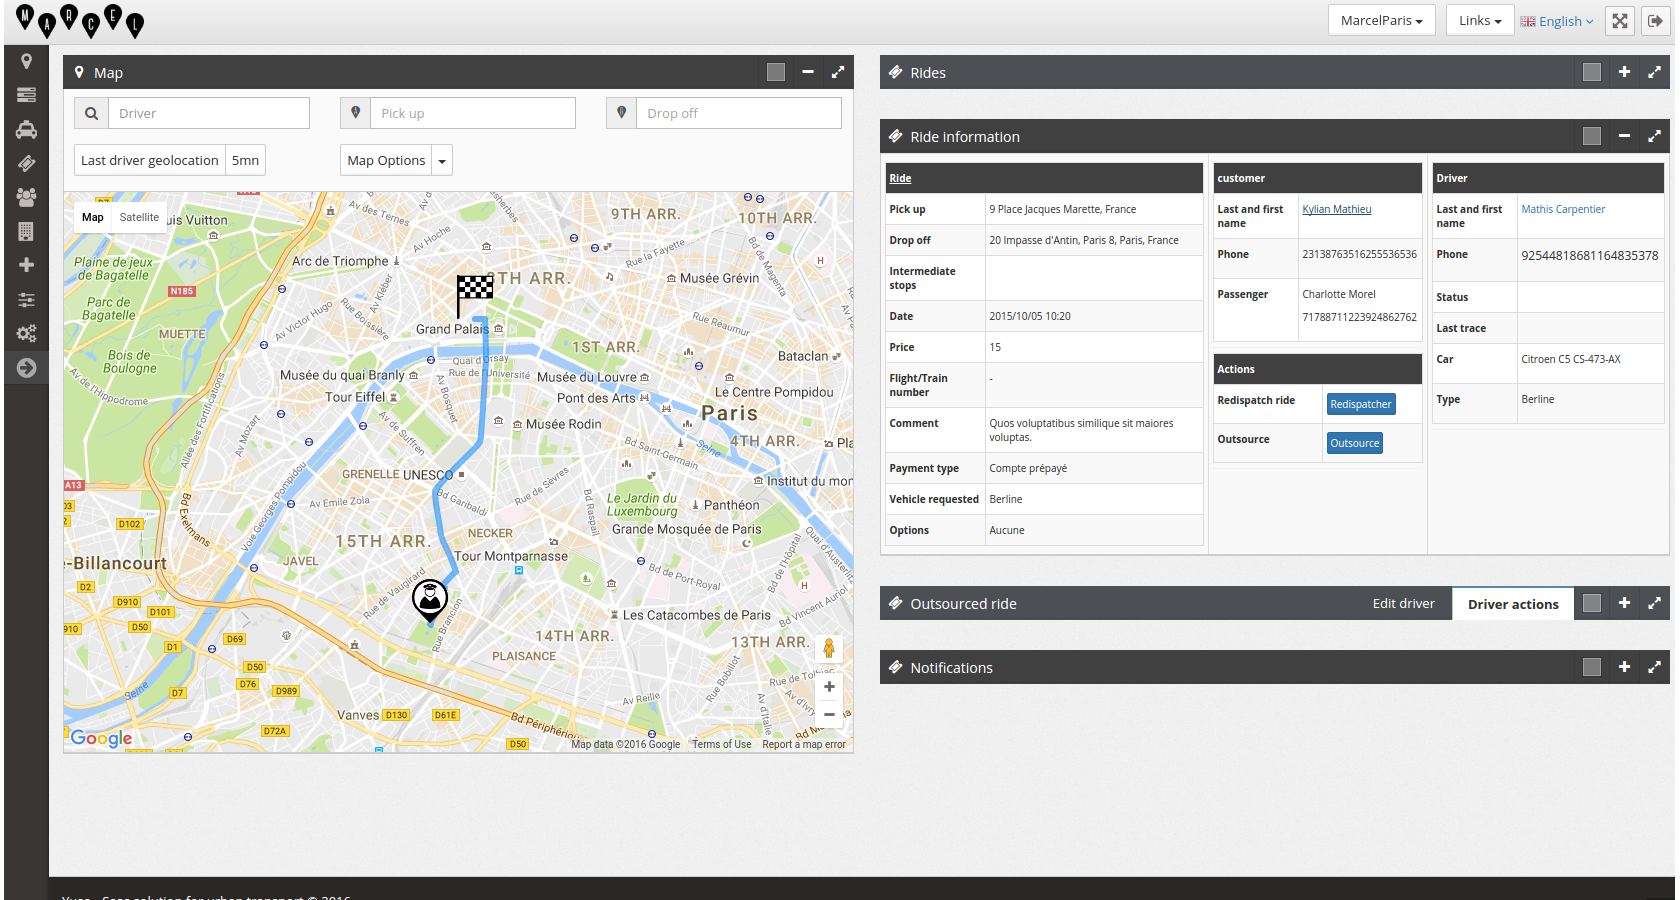
\includegraphics[width=6 in]{images/achievement/6.png}
\caption{Interface of the ride's information display }
\label{int6}
\end{center}
\end{figure}

\newpage


\subsection{Live Drivers}

The main aspect of our application is to control and view drivers in real time, hence, the user owns the entitlement of observing geolocated drivers. In fact, the drivers are being constantly geolocated through the same solution.

Meanwhile, their positions are shows as markers on the map of the all of the members of their SaaS company. Figure \ref{int1} is all about the map filled with dispersed pins. Those pins represent the drivers according to their specification.

~

\begin{figure}[!htbp] 
\begin{center}
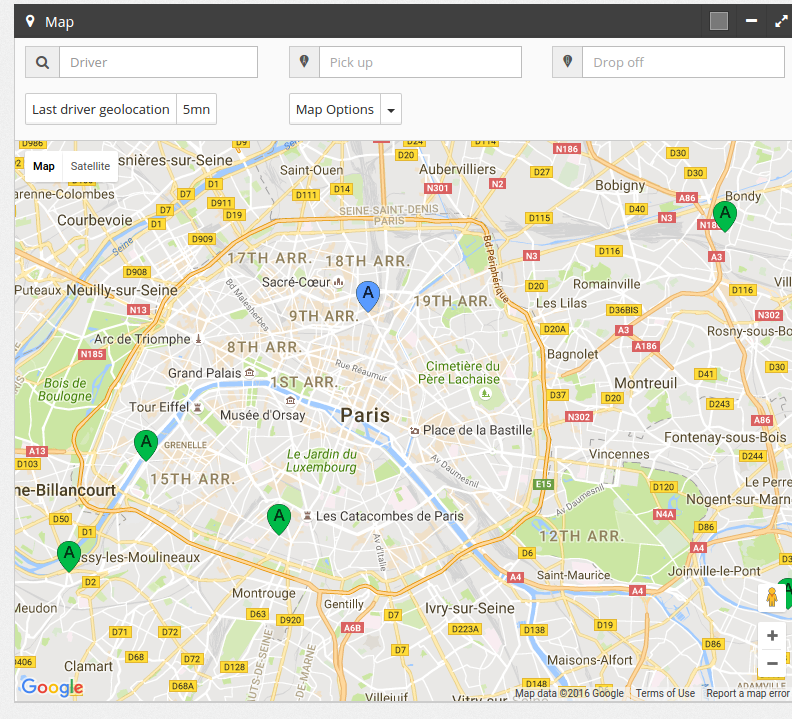
\includegraphics[width=6 in]{images/achievement/1.png}
\caption{Interface of the map with live drivers}
\label{int1}
\end{center}
\end{figure}~

The pins change their positions as the geolocalization is a continuous process. Every second the pins are alternated following the recent characteristic collected from the server. An overview of some rules are summarized in Table 5.2. The colors are standard for each client. Nevertheless, the letter written on the pin depends on the vehicle's type.



\begin{table}[!htbp]
\begin{center}
\noindent\begin{tabular}{| m{33em} | m{2cm} | }
\hline
Status & Pin \\
\hline
Started & 
\includegraphics[width=0.2 in]{images/pins/started.png} \\ 
Available & 
\includegraphics[width=0.2 in]{images/pins/dispo.png}  \\ 
Unavailable & 
\includegraphics[width=0.2 in]{images/pins/indispo.png}  \\ 
Accepted & 
\includegraphics[width=0.2 in]{images/pins/accepted.png}  \\ 
On the way & 
\includegraphics[width=0.2 in]{images/pins/way_to.png}  \\ 
On hold & 
\includegraphics[width=0.2 in]{images/pins/wait.png} \\  
Pause  & 
\includegraphics[width=0.2 in]{images/pins/pause.png}  \\ 
Soon-to-clear & 
\includegraphics[width=0.2 in]{images/pins/soon-to-clear.png}  \\  
Selected &  
\includegraphics[width=0.2 in]{images/pins/selected.png}   \\ 
Not dispatched/ Dispatched/ Dispatched Frozen/ Affected & 
\includegraphics[width=0.2in]{images/pins/not_dispatched-dispatched-dispatched_frozen-affected.png} \\ 
\hline
\end{tabular}
\end{center}
\label{pins}
\caption{Types of drivers' markers}
\end{table}




After surveying the markers, the user has also the possibility of selecting a single pin to the extend of displaying further information. As Figure \ref{int7} exhibits, a small box is displayed in the bottom of the map, listing some basic information about the driver, as well as the last geolocation time. Moreover, the color of the selected pin is changed with the preservation of the previous color. The focused pin is then highlighted and the map is zoomed around its range zone. 

Besides, the box may be hidden by a simple deselection of the chosen pin. But also, the possibility of selecting another pin while the box is active is also available. In that case, the information are changed instantly according to the new pin, and the new pin is highlighted and zoomed in like the previous one.
The old pin retrieves then its previous color either way.

\begin{figure}[!htbp] 
\begin{center}
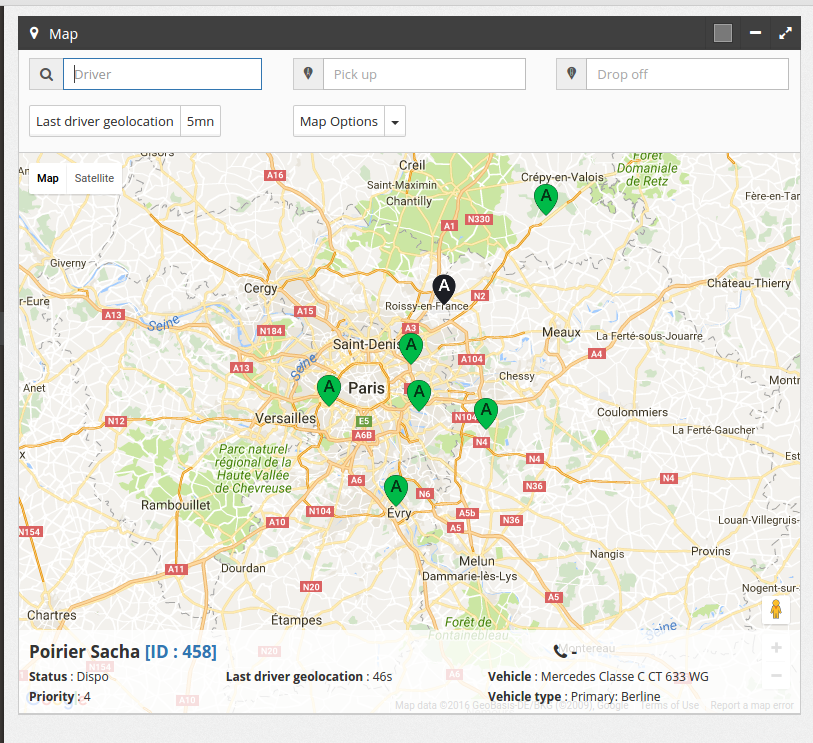
\includegraphics[width=5.8 in]{images/achievement/7.png}
\caption{Interface of the map with a selected driver}
\label{int7}
\end{center}
\end{figure}

\newpage


A few other options are mandatory in order to retrieve live driver quickly. Actually, the user may filter the driver by their last geolocation time. A menu composed of certain time intervals is available in order to hide the pins of the drivers that exceeded the time set by the user. However, pins that match the requirement are instantly shown on the map.

Furthermore, the user may search for specific set of pins by inserting various arguments. The user may input the driver's name, the pick-up and the drop-off addresses. For instance, Figure \ref{int8} demonstrates a research by the name of 'Henry'. The only marker left is by the name of Henry and has been geolocated for 37 seconds which is less than 5 minutes.

~

\begin{figure}[!htbp] 
\begin{center}
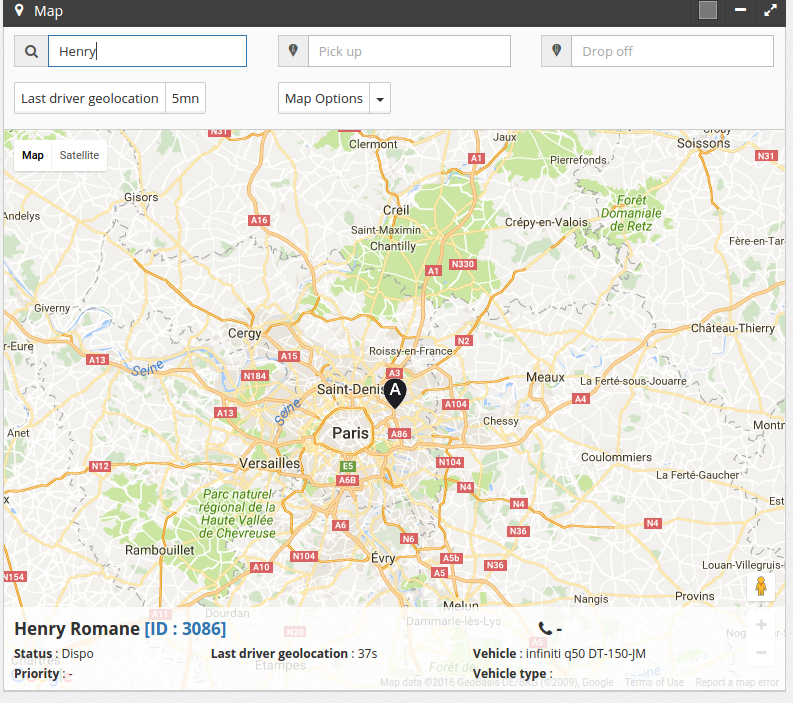
\includegraphics[width=6 in]{images/achievement/8.png}
\caption{Interface of map with filtered driver}
\label{int8}
\end{center}
\end{figure}~

~~


To wrap things up, each feature will not reduce the efficiency of an other feature, owing to the fact that, the implementation process made sure that they can work together in a harmony. Parallel procedures may occur without the need to worry about misleading results. And finally, the system has the capability to perform all of the operations simultaneously in order to provide faster and more precise information to the user.

\subsection *{Conclusion}
During this chapter, we presented the technologies that were chosen to implement our project and we argued that choice. We also presented the framework that was used and we finished by displaying the main features and interfaces of our application.



